\documentclass[10pt]{article}
\usepackage[a4paper, tmargin=0.75in, lmargin=0.80in, rmargin=0.80in, bmargin=1in]{geometry}
\usepackage{hyperref}


\usepackage{graphicx}
\pagestyle{empty}
\usepackage{xcolor}
\usepackage{subfig}

\begin{document}
	
	\begin{center}
		{\Huge{Computer Vision Assignment}} \\
		\vspace{2mm}
		
	\end{center}
	\section*{\textcolor{blue}{Datasets}}
	\subsection{COCO }
	The \textbf{Common Objects in Context (COCO)} dataset is a large-scale benchmark dataset developed by Microsoft. It contains over 200,000 labeled images and more than 80 object categories with instance segmentation, keypoint annotations, and captioning.
	
	\begin{itemize}
		\item \textbf{Classes:} 80 object categories
		\item \textbf{Annotations:} Bounding boxes, segmentation masks, keypoints
		\item \textbf{Use case:} General-purpose object detection and segmentation
		\item \textbf{Format:} JSON annotations in COCO format
	\end{itemize}
	
	COCO is commonly used to pretrain deep learning object detectors such as Faster R-CNN, RetinaNet, and YOLO. It features complex scenes with multiple objects and varying scales.
	\subsection{Pascal VOC}
	\textbf{Pascal VOC (Visual Object Classes)} is a benchmark dataset for object detection, segmentation, and classification. The most commonly used versions are VOC 2007 and VOC 2012.
	
	\begin{itemize}
		\item \textbf{Classes:} 20 object categories (subset of COCO classes)
		\item \textbf{Annotations:} XML files with bounding boxes and labels
		\item \textbf{Use case:} Lightweight evaluation and fine-tuning
		% \item \textbf{Evaluation:} Mean Average Precision (mAP) at IoU = 0.5
	\end{itemize}
	
	Pascal VOC is widely used for academic benchmarking, especially for models trained on smaller datasets or when COCO’s scale is unnecessary.
	\section*{\textcolor{blue}{Models}}
	\subsection{RetinaNet}
	\textbf{RetinaNet} is a one-stage object detection model. It addresses the foreground-background class imbalance by introducing the novel \textbf{focal loss} function.
	
	\begin{itemize}
		\item \textbf{Backbone:} ResNet-50 or ResNet-101 with Feature Pyramid Network (FPN)
		\item \textbf{Architecture:} One-stage detector with dense anchors
		\item \textbf{Loss function:} Focal loss to reduce background dominance
		\item \textbf{Advantages:} Faster than two-stage models like Faster R-CNN, while maintaining high accuracy
	\end{itemize}
	
	In our assignment, we used a \textbf{COCO-pretrained RetinaNet} and evaluated its performance on the VOC 2012 validation set. Evaluation was done using \texttt{torchmetrics}'s \texttt{MeanAveragePrecision} metric at an IoU threshold of 0.5.
	
	
	\section*{\textcolor{blue}{Evaluation Summary}}
	\subsection*{\textcolor{red}{RetineNet}}
	\subsubsection*{{COCO Dataset}}
	After running inference on the COCO validation set, the following results were obtained:
	
	\begin{itemize}
		\item \textbf{mAP@0.5:0.95} 0.4151
		 
		 \item \textbf{mAP@0.5} 0.618
		\item \textbf{mAP@0.75} 0.4391
	\end{itemize}
	
	\subsubsection*{{VOC Dataset}}
	After running inference on the VOC 2012 validation set, the following results were obtained:
	
	\begin{itemize}
		\item \textbf{mAP@0.5:} 0.585
		
		\item \textbf{Best performance:} Large objects
		
	\end{itemize}
	\begin{figure}[h]
		\centering
		\subfloat[\centering Failure]{{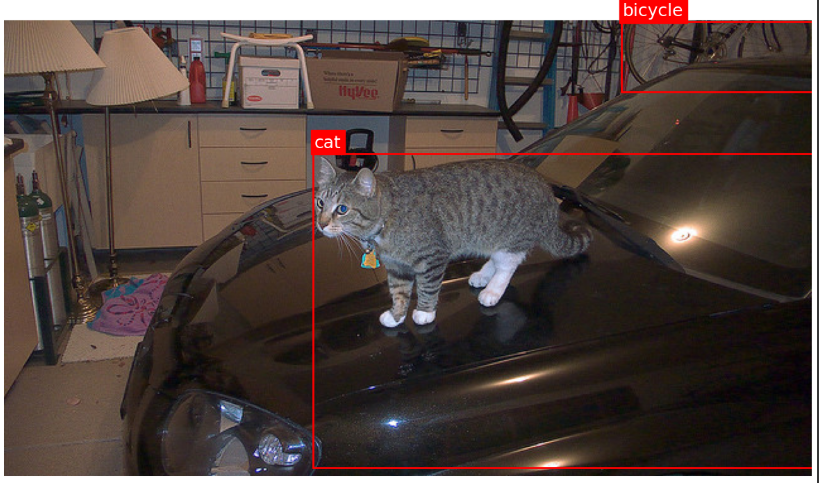
\includegraphics[width=5cm]{coco_f1.png} }}%
		\qquad
		\subfloat[\centering Success]{{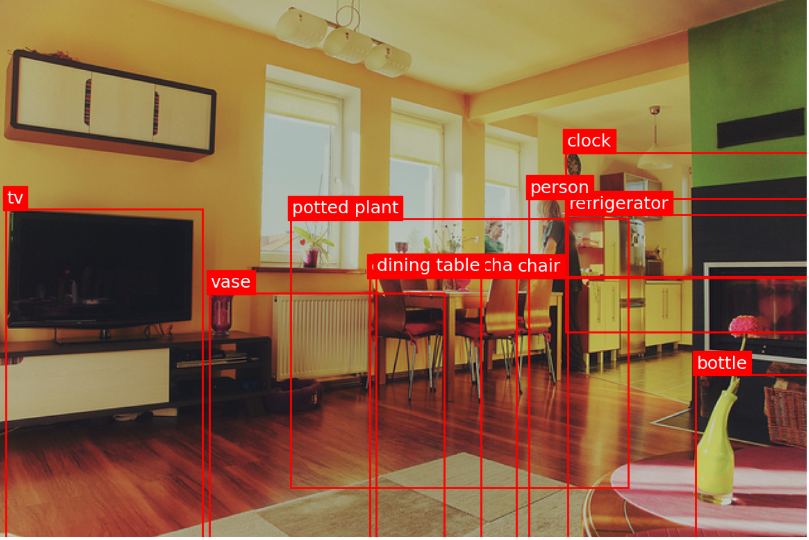
\includegraphics[width=5cm]{coco_s1.png} }}%
		\caption{COCO Test Cases}%
		
	\end{figure}
	
	
	
	\begin{figure}[h]
		\centering
		\subfloat[\centering Failure]{{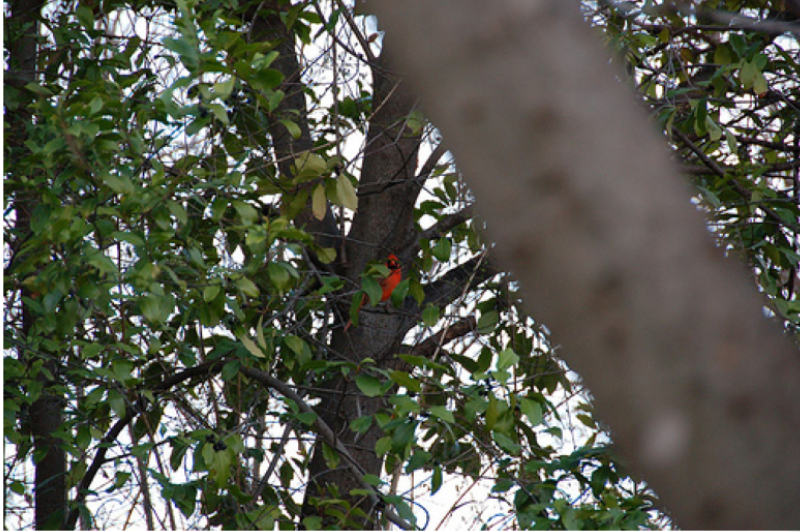
\includegraphics[width=5cm]{voc_f1.png} }}%
		\qquad
		\subfloat[\centering Success]{{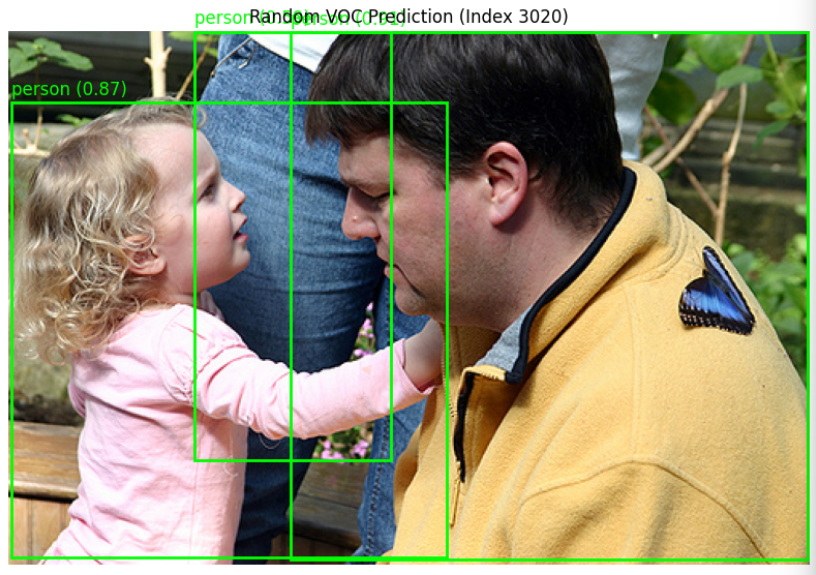
\includegraphics[width=5cm]{voc_s1.png} }}%
		\caption{VOC Test Cases}%
		
	\end{figure}
	
	
	
	
	\newpage
	\bibliographystyle{aasjournal}
	\bibliography{references}{}
	
	
\end{document}
